\chapter{Lecture 5 - Applied Perception II}
Color is extremely useful in data visualization to show patterns, for labeling, and for highlighting. However, color is easy to misuse. Think of "color" as an attribute of an object rather than its primary characteristic. 

\section{Basic color perception}
Human have three distinct color receptors on the retina, called the \textit{cones}, which are active at normal light levels. With the support of rods on color perception, we can perceive light or a "shadowy figure" in low luminosity conditions.

\begin{definition}[Trichromacy theory]
    Cones are sensitive to different wavelengths(short, medium, long), hence, they absorb light around the spectrum of \emph{blue, green, and red}. The theory says that we perceive color as a three-channel system. \par
    All color spaces, even if designed to different purposes, as three-dimensional.
\end{definition}

\begin{figure}[htbp]
    \centering
    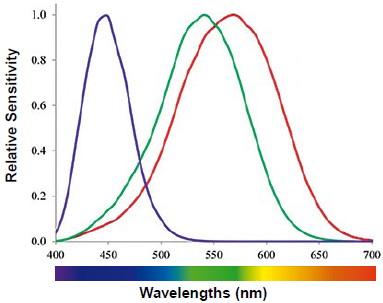
\includegraphics[width=0.3\linewidth]{imgs/lecture5/5.1 thrichromacy theory.png}
    \caption{Thrichromacy theory}
    \label{fig:5.1}
\end{figure}

\subsection{Color measurement and specification}
Since only three different receptors are involved in color vision, it is possible to match a patch of color light using a mixture of three color lights, called \emph{primaries}. The color experiment consists in using a transformation to create the same color on different output devices. \par
In fig~\ref{fig:5.2a} we show the experiment setup and results, the goal of the experiment is represented in "making screen", adjust the colors so that the two halves of the circle show the same color.\par
In fig~\ref{fig:5.2b} we show the experiment result on how sensitive our eyes perceive the primaries, the so-called \textbf{RGB color space}, created by the CIE - International Commission of Color.

\begin{figure}[htbp]
    \centering

    \begin{subfigure}[b]{0.4\linewidth}
        \centering
        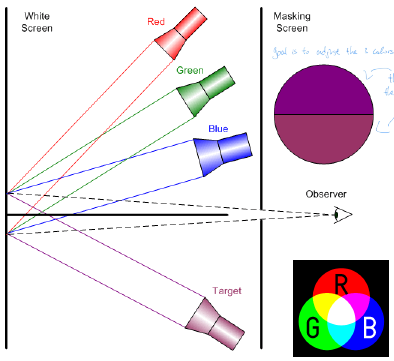
\includegraphics[width=\linewidth]{imgs/lecture5/5.2 color experiment.png}
        \caption{Experiment setup}
        \label{fig:5.2a}
    \end{subfigure}
    \hfill
    \begin{subfigure}[b]{0.4\linewidth}
        \centering
        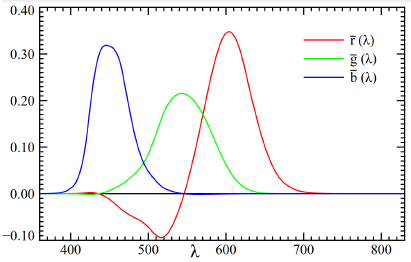
\includegraphics[width=\linewidth]{imgs/lecture5/5.3 color results.png}
        \caption{Experiment results as functions}
        \label{fig:5.2b}
    \end{subfigure}

    \caption{Color measurement experiment}
    \label{fig:5.2}
\end{figure}

The RGB color matching function can also be represented as a \textit{function of X, Y, and Z}, where:
\begin{itemize}[noitemsep]
    \item Y corresponds to the perceived luminance in well-lit condition
    \item Z is close to the short cone response
    \item X is a mix such that the values become non-negative
\end{itemize}
And for a fixed value of Y, the plane XZ contains all the possible chromaticities at that luminance.

\begin{figure}[htbp]
    \centering

    \begin{subfigure}[b]{0.4\linewidth}
        \centering
        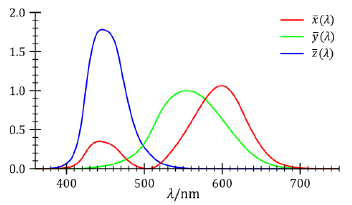
\includegraphics[width=\linewidth]{imgs/lecture5/5.4 xyz color matching.png}
        \caption{Color matching function as XYZ}
        \label{fig:5.3a}
    \end{subfigure}
    \hfill
    \begin{subfigure}[b]{0.4\linewidth}
        \centering
        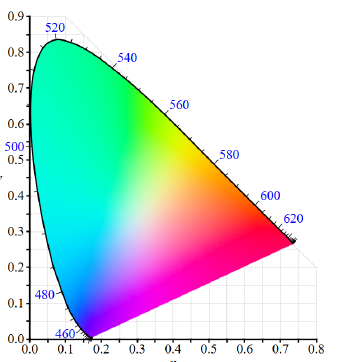
\includegraphics[width=0.5\linewidth]{imgs/lecture5/5.5 chromaticity diagram.png}
        \caption{Chromaticity diagram}
        \label{fig:5.3b}
    \end{subfigure}

    \caption{XYZ color space}
    \label{fig:5.3}
\end{figure}

\begin{definition}[Gamut]
    Gamut is the set of color spaces that a device, such as a printer or a monitor can reproduce. Most of the time, it is a subspace of the chromaticity diagram
\end{definition}

\subsection{Opponent process theory}
The theory was proposed by Hering, a German psychologist, and later supported by experiments. Hering proposed that cones combine their stimulus, forming three pairs of colors that compete to form the final one. These pairs, called \emph{opponent pairs} are \emph{black-white, red-green, and yellow-blue}.\par
This theory suggests that the visual system interprets color by processing signals from three types of cone cells in an antagonistic manner, meaning that the activation of one color inhibits the perception of its opposite.\par
One interesting implication is the \emph{afterimages}. For example, if you stare at a bright color (like red) for a long period of time and then look at a white-colored surface, you may see a cyan afterimage. This happens because the red receptors become fatigued, leading to the perception of their complementary color. \par 
It also suggests the extremes of the opponent channels, which are fundamental to our understanding of color perception. These unique hues are \emph{red, green, blue} which cannot be created by mixing other colors.

\begin{figure}[htbp]
    \centering
    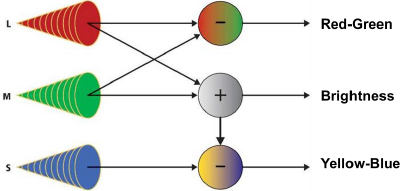
\includegraphics[width=0.4\linewidth]{imgs/lecture5/5.6 opponent process theory.png}
    \caption{Opponent process theory}
    \label{fig:5.4}
\end{figure}

In fig~\ref{fig:5.5} shows an example of this theory in practice. When looking at this picture for at least 30 seconds, and focus at the little white dot in the middle. Then switch to a white colored surface, and what we see on the white background is the flag of the USA. This is because when you stare at these colors, you are exciting the same source of these colors, and when you switch to the white background, since these sensors have been excited for too long, they inhibit those colors as the only colors.

\begin{figure}[htbp]
    \centering
    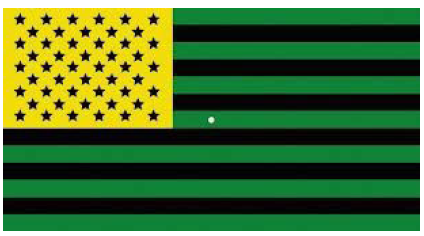
\includegraphics[width=0.3\linewidth]{imgs/lecture5/5.7 opponent process theory-example.png}
    \caption{Opponent process theory, an example}
    \label{fig:5.5}
\end{figure}

\section{Color spaces}
\textbf{Saturation} means how pure the color is, intended as its brightness.

\begin{figure}[htbp]
    \centering
    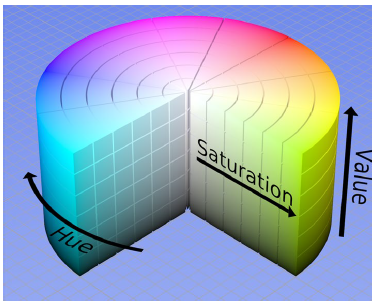
\includegraphics[width=0.3\linewidth]{imgs/lecture5/5.8 hue saturation values.png}
    \caption{Hue Saturation Value}
    \label{fig:5.6}
\end{figure}

Color specification can be represented as in fig~\ref{fig:5.6}, which is a more natural representation than with RGB. But, they are not perceptually uniform spaces (calculated Euclidean distance in the color space does not correspond to perceptual distances).\par
Having a color space in which equal perceptual distances are useful to specify color tolerances, color codes, pseudo-coloring using sequences of colors to represent data values, possibly with perceptually equal steps.\par

The Euclidean distance is meaningful from a perceptual point of view for the color space. It is defined in eq~\ref{eq:5.1}.
\begin{equation}
    \Delta E_{ab}^{*} = \sqrt{(L_2^{*} - L_1^{*})^2 + (a_2^{*} - a_1^{*})^2 + (b_2^{*} - b_1^{*})^2}
    \label{eq:5.1}
\end{equation}

If the result \(\Delta E\) < 1, colors are not perceptible; for 1 < \(\Delta E\) < 2, close observation needed to perceive the difference; for 2 < \(\Delta E\) < 10, the colors are similar but different. It is important to know that \(\Delta E\) is not perceptually uniform as originally intended and therefore suspended by specifications.\par
Although uniform color spaces only provide a rough first approximation of how color differences will be perceived, an important influencing factor is size: we are much more sensitive to differences between large patches. \par
\textit{Tips}: Use saturated colors when coding small symbols or thin lines, and less saturated colors for large areas, as showed in fig~\ref{fig:5.7}.

\begin{figure}[htbp]
    \centering
    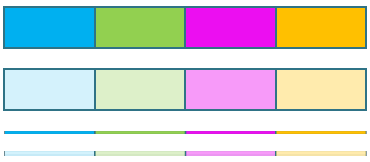
\includegraphics[width=0.3\linewidth]{imgs/lecture5/5.9 color differences.png}
    \caption{Color differences and use of saturation}
    \label{fig:5.7}
\end{figure}

\section{Color and Visualization}
The red-green and yellow-blue chromatic channels presented from the opponent process theory are each capable of carrying only about 1/3 of the amount of detail carried by the black-white channel.\par
Purely chromatic differences are not enough to display fine details, ensuring adequate luminance contrast with the background, and also colors with different chromaticity (saturation) can be used to improve readability.

\begin{figure}[htbp]
    \centering

    \begin{subfigure}[b]{0.4\linewidth}
        \centering
        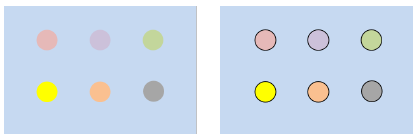
\includegraphics[width=\linewidth]{imgs/lecture5/5.10 visualization and luminance.png}
        \caption{Contrast boundary to improve readability}
        \label{fig:5.8a}
    \end{subfigure}
    \hfill
    \begin{subfigure}[b]{0.4\linewidth}
        \centering
        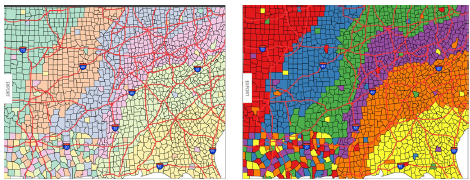
\includegraphics[width=\linewidth]{imgs/lecture5/5.11 visualization and saturation.png}
        \caption{Less saturated colors for large patches and saturated colors for finer details}
        \label{fig:5.8b}
    \end{subfigure}

    \caption{Visualization and color properties}
    \label{fig:5.8}
\end{figure}

In 1986, Post and Greene carried out an experiment on the naming of colors; among 210 different colors, only 8, plus white, were consistently named. This result suggests that only a few colors can be used as categorical labels. Nowadays, the 12 recommended colors shown in fig~\ref{fig:5.9} are widely agreed-upon category names with reasonably far apart in color space. These colors are: red, yellow, black, pink, gray, brown, green, blue, white, cyan, orange, purple.

\begin{figure}[htbp]
    \centering
    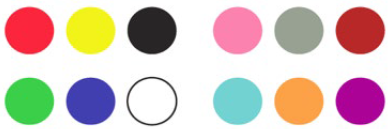
\includegraphics[width=0.3\linewidth]{imgs/lecture5/5.12 color labels.png}
    \caption{Color labels}
    \label{fig:5.9}
\end{figure}

\subsubsection{Color and Semantics}
There are no universal conventions on associating a color with some semantics, but they are widely used. For instance, red for hot/bad/danger, blue for cold, green for life/go, etc. The semantic association with gray is that of belonging to an unspecified category, which can be used for highlighting more important information using different colors. 

\subsubsection{Color ramps}
Color ramps are a predefined set of colors used to present a theme (green-yellow hue of colors represents summer, red-orange-yellow hue of colors represents autumn ...).\par
There are some guidelines in using color ramps, for instance, avoid color ramps problematic for color-blind individuals; use a spectrum-based color ramp when its use is deeply embedded in the user culture; to reveal fine details, use a pseudo-color sequence that varies in luminance, not only in chromaticity. 